\documentclass[journal=jprobs,manuscript=article]{achemso}

\usepackage[version=3]{mhchem} % Formula subscripts using \ce{}
\usepackage[T1]{fontenc}       % Use modern font encodings
\usepackage{multirow}

\newcommand*\mycommand[1]{\texttt{\emph{#1}}}

\author{Stefan K. Solntsev}
\email{solntsev@wisc.edu}
\author{Michael R. Shortreed}
\author{Brian L. Frey}
\author{Lloyd M. Smith}
\affiliation[UwMadison]
{University of Wisconsin-Madison}

\title[Rapid and Accurate Global PTM Discovery (G-PTM-D) Using Post-Acquisition Spectral Calibration and Defined Mass Windows]
  {Rapid and Accurate Global PTM Discovery (G-PTM-D) Using Post-Acquisition Spectral Calibration and Defined Mass Windows}

\begin{document}

\begin{abstract}

Correct identification of protein posttranslational-modifications (PTMs) is crucial to understanding many aspects of protein function in biological processes.
G-PTM-D\cite{Li_2016} is a recently developed tool for global identification of PTMs.
Spectral file calibration prior to applying the tool, and algorithmic improvements in the peptide database search greatly improve the accuracy and efficiency of PTM identification.
We enhanced G-PTM-D by using targeted mass-window searches, and demonstrate its effectiveness in identification of numerous types of PTMs, including high-mass modifications such as glycosylations.
The proposed changes lead to a 20\% increase in the number of identified modifications and an order of magnitude decrease in the search time.
Additional advantages of using targeted mass-windows searches in context of novel modification discovery are shown.
\end{abstract}

\section{Introduction}

Many peptide residue modification types are known, and databases containing detailed information about such modifications are readily available.
Information about a modification can include the chemical or isotopic composition, mass, specificity to certain residues, and possible restriction of placement to peptide or protein termini.
While this data is almost comprehensive, information about the localization of these modification to certain residues in specific proteins is scarce.

A recently described bioinformatics tool for the discovery and localization of new PTMs from "bottom-up" tandem mass spectrometric datasets, G-PTM-D\cite{Li_2016} is the foundation for the work described in this paper.
The G-PTM-D workflow consists of three stages: 1) A wide-mass database search\cite{Chick_2015,Na_2011} that provides spectral matches to unmodified peptides along with the mass differences between the identified peptides and the measured parent peptide masses (hypothesized to differ in mass due to the presence of a PTM).
2) For those peptides for which the mass difference corresponds to the mass of a known PTM, a database augmentation step adds plausible localized PTMs to the proteins in the search database.
3) A final standard narrow-mass search of the augmented database to identify both modified and unmodified peptides subject to the standard FDR threshold (e.g. 1\% FDR).

Before describing the proposed changes to G-PTM-D, a few definitions of the various search modes must be introduced.
A standard \textit{narrow-mass} search considers matching theoretical peptides to spectra if the peptide mass and the identified precursor mass are equal, within some tolerance (i.e. 5ppm, or 2.1 Da).
A \textit{wide-mass} search matches peptide fragment masses to fragmentation spectra while allowing large differences (i.e. $\pm 500$ Da) between the observed precursor mass and the peptide mass.
An even less restrictive \textit{open-mass} search, matches peptides from a database to fragmentation spectra without taking the precursor mass into account.
We propose alternatives to these search modes, namely a \textit{notch search} and an \textit{interval search} that fall under a broad category of \textit{mass-window} searches.
The notch search is an extension of the narrow-mass search: it allows exact matches (within a tolerance) to specific mass differences between the theoretical peptide and observed precursor masses.
The interval search is an extension of the wide-mass search: specific problematic mass differences are excluded from allowed matches.
The smaller the fraction of the mass space, and the narrower the mass window per search element, the faster the search will run (as fewer searches are executed per mass spectrum).
Figure~\ref{fgr:differentSearchModes} provides a convenient way to visualize the various search modes.

We propose an extension to G-PTM-D (Enhanced G-PTM-D) that addresses the long search times of the wide-mass search, and the limitations of the standard final narrow-mass search.
The wide-mass search is replaced by a notch search in the discovery phase, using notches centered at the monoisotopic mass differences introduced by known modifications.
This change improves the specificity and significantly decreases search time.
The final narrow-mass search is also replaced by a notch search, further increasing the number of confidently identified peptides.

The mass-window search is useful in other procedures as well, beyond the G-PTM-D workflow.
Its efficacy is demonstrated in context of a search for novel modifications, which is usually based on a wide-mass or an open-mass search.
A combination of specialized notch and interval searches produces superior identification and discovery results.

Along with algorithmic improvements, spectral calibration prior to running the G-PTM-D procedure is essential.
A critical parameter for peptide identification and PTM localization is mass accuracy\cite{Scherl_2008}.
Higher mass accuracy provides increased specificity and thus confidence in peptide identifications, decreasing the false discovery rate.
Instrument noise, systemic drift and miscalibration limit the mass accuracy in acquired spectra.
Multiple calibration strategies to improve mass accuracy have been devised, and fall into three general categories:  External calibration prior to the MS experiment (e.g. standard instrument calibration protocols); internal calibration during the MS experiment (e.g. real-time calibration using a lock mass standard\cite{Olsen_2005}); and subsequent to the MS experiment (post-acquisition spectral calibration, REF).
We use a post-acquisition calibration procedure, that builds upon the software lock mass concept\cite{Cox_2011} recently reported by the Mann group.
In our strategy, the m/z differences between expected and observed peaks in the peptide tandem ms spectra are compiled, and then used to recalibrate the spectra.
The increased mass accuracy of the recalibrated spectra leads directly to improved identifications of both modified and unmodified peptides, as well as to increased confidence for PTM localization.

\begin{figure}
  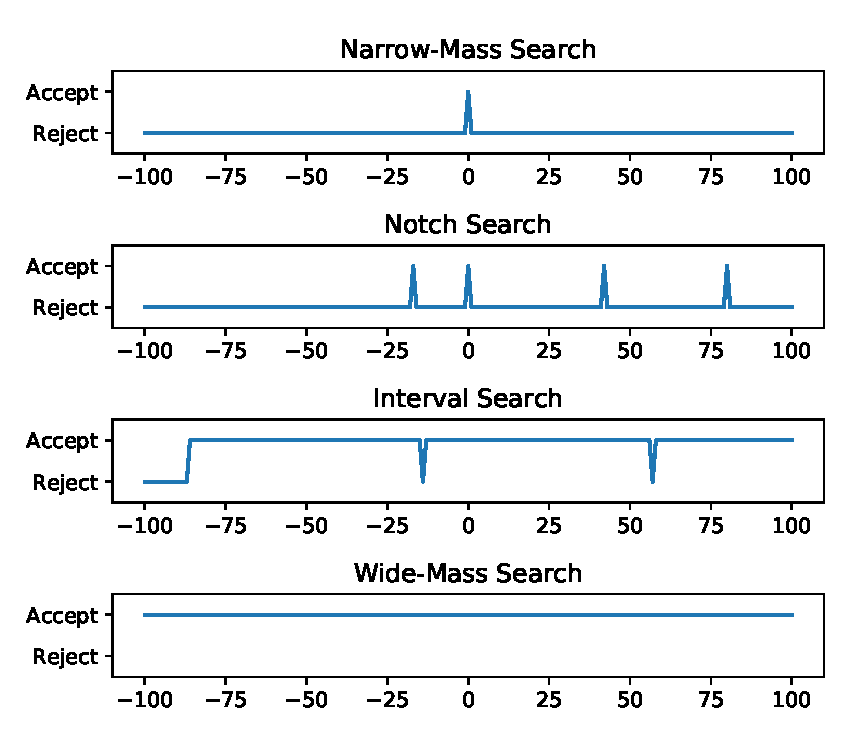
\includegraphics{figureDifferentSearchModes.eps}
  \caption{Search Modes}
  \label{fgr:differentSearchModes}
\end{figure}

\section{Experimental Procedures}
We developed a modified version of the Morpheus software for bottom-up spectral database searching\cite{Wenger_2013} that we call MetaMorpheus, which integrates the database search procedure with spectral calibration and the Enhanced G-PTM-D workflow.
Two multi-fraction mammalian datasets (\textit{Mouse} and \textit{Jurkat}) with deep proteome coverage were used to evaluate the performance of the methods: these datasets are described in detail in~\cite{Shortreed_2015, Cesnik_2016}.
Uniprot XML protein databases acquired on Feb 27, 2017 containing only reviewed human/mouse proteins were employed. 

A 10ppm precursor mass tolerance was used for the initial calibration step, and then reduced to 5ppm for subsequent notch searches.
For the database augmentation step, we allowed 120 modifications including PTMs, adducts, and chemical modifications.
Final notch search used notches centered at \{0, 1.003, 2.005, 3.008\} in order to capture missed identifications due to missed monoisotopic peaks.

For the discovery of novel modifications, we used a combination of two searches: A notch search with notches at all combinations of up to 2 residue mass additions or removals, and an interval search with lower bound of -187 Daltons, and with exclusions at masses corresponding to the notch search.

\section{Results and Discussion}

The input into the workflow is a standard bottom-up tandem-MS dataset obtained from a tryptically digested protein sample along with a corresponding protein sequence database, and the output is a comprehensive set of peptide and PTM identifications.
 
\subsection{Enhanced G-PTM-D}

By employing the novel notch search strategy instead of the wide-mass search in the G-PTM-D process, using only the modifications listed in Uniprot, the number of confidently identified PSMs increased by 6\%.
The overall search time dropped significantly, from 35 hours to 4 hours for all datasets, see Table~\ref{my-label}.

\begin{table}[]
\centering
\caption{Effects of Replacing Initial Wide-Mass Search by a Notch Search}
\label{my-label}
\begin{tabular}{ll|l|l}
                      &        & Wide-Mass Search & Notch Search\\
\hline
\multirow{2}{*}{Time} & Jurkat & 22.1 hrs         & 2.9 hrs    \\
                      & Mouse  & 13.5 hrs         & 1.2 hrs   \\
\hline
\multirow{2}{*}{PSMs} & Jurkat & 203237           & 210566    \\
                      & Mouse  & 153674           & 162473   
\end{tabular}
\end{table}


The final search with the augmented database is conducted with notches: we only recommend including the common missed monoisotopic mass values in the final search,.
The effect of using these notches is shown in Table~\ref{tab:table2}.

\begin{table}[]
\centering
\caption{Effects of Replacing Final Narrow-Mass Search by a Notch Search}
\label{tab:table2}
\begin{tabular}{ll|l|l}
                      &        & Narrow-Mass Search & Notch Search\\
\hline
\multirow{2}{*}{PSMs} & Jurkat  & 210566   &  220574  \\
                      & Mouse    & 162473   &   170743
\end{tabular}
\end{table}

Since the XML database is annotated with PTMs from the UniProt PTM list, it is natural to use it in the augmentation step as well.
It has a few significant drawbacks: Some mass values do not correspond to actual mass shifts, lability of modifications is not taken into account, and many PTMs are missing, including adducts and glycosylations.
Notch searches allow using expanded modification lists that include chemical modifications such as adducts and large mass PTMs such as glycosylations.
Even though adducts arising from experimental artifacts are not ultimately interesting to biologists, not including them as an option decreases the total number of identified proteins and PTMS.
A curated set of notches and the corresponding modifications is given in Appendix A.
The overall identification rate increased from 164,697 to 179,345 peptide-spectral matches (PSMs), which in turn increased the number of modified peptides by an additional 20\%.
We identified hundreds of glycosylated peptides in these unenriched samples, with many of these modifications exceeding 1000 Daltons. 

\begin{table}[]
\centering
\caption{Effects of Using Different Modification Lists}
\label{tab:table3}
\begin{tabular}{ll|l|l|l}
                      &        & Only Uniprot & Uniprot+Glyco & Uniprot+Glyco+Adducts\\
\hline
\multirow{2}{*}{PSMs} & Jurkat  & 220574   &  222985 & 223578\\
                      & Mouse    & 170743   &   171432& 174783 
\end{tabular}
\end{table}


\subsection{Mass Windows in an Open Search}

Restricting the allowed precursor masses is beneficial in searches that are intended to discover mass shift peaks.
We ran a completely open precursor mass search, and restricted ourselves to looking at 1\% FDR matches, both targets and decoys.
The plots in Figure~\ref{fig:figure2-upperlowerbounds} show the FDR in the list filtered by using a lower or upper bound cutoff on the allowed mass shifts.
It shows the fundamental difference between upper and lower bound cutoffs: while it is beneficial to restrict open searches to ignore large negative values, restricting matches with a large positive mass difference has a negative effect on the overall FDR.

This effect can be explained by the fact that it's easier to match long sequences to short peptide fragmentation profiles than it is to match short sequences to fragmentation pattern of a long peptide.

\begin{figure}
\caption{Upper and Lower bound cutoffs in Mouse Data}
\label{fig:figure2-upperlowerbounds}
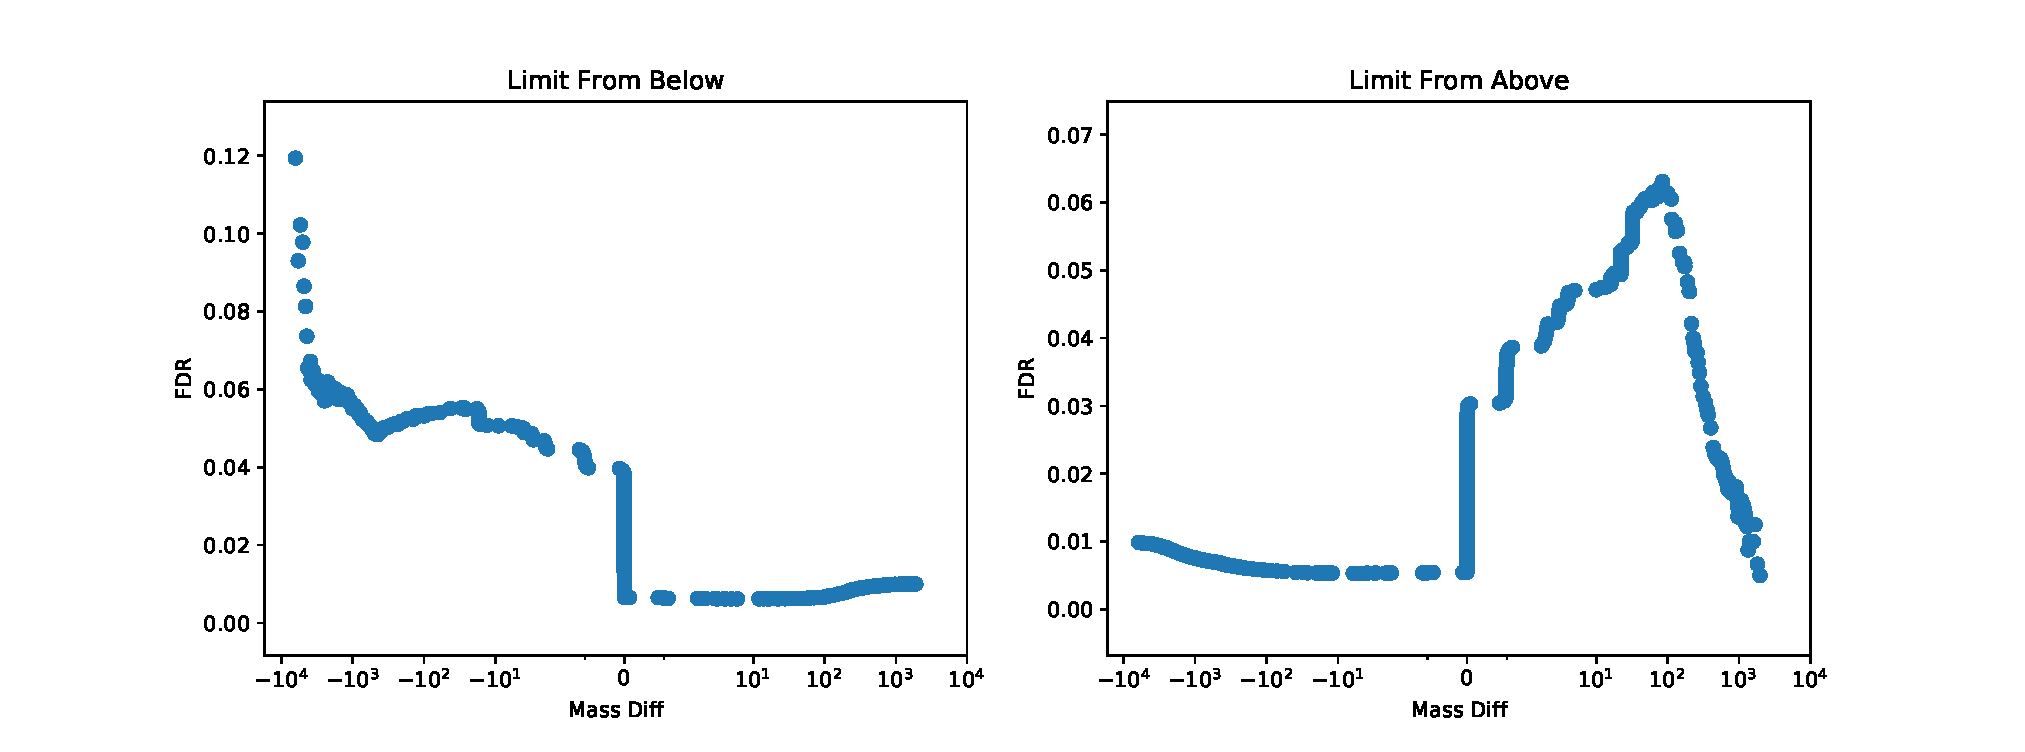
\includegraphics[scale=0.5]{figure_2-upperlowerbounds}
\end{figure}

MetaMorpheus includes a capability to identify peaks in a mass shift histogram obtained from a search, using a recently described peak finding algorithm\cite{Rodriguez_2014}.
We identified peaks with anomalously high false discovery rates, which could be excluded from wide mass searches in order to improve the overall identification quality.
Some histogram peaks are illustrated in Figure~\ref{fig:figure3}, including peaks corresponding to masses of Sulfo and Phospho, and a problematic peak at mass of Leucine, with a high FDR.

\begin{figure}
\caption{Some Histogram Peaks For Mouse Data}
\label{fig:figure3}
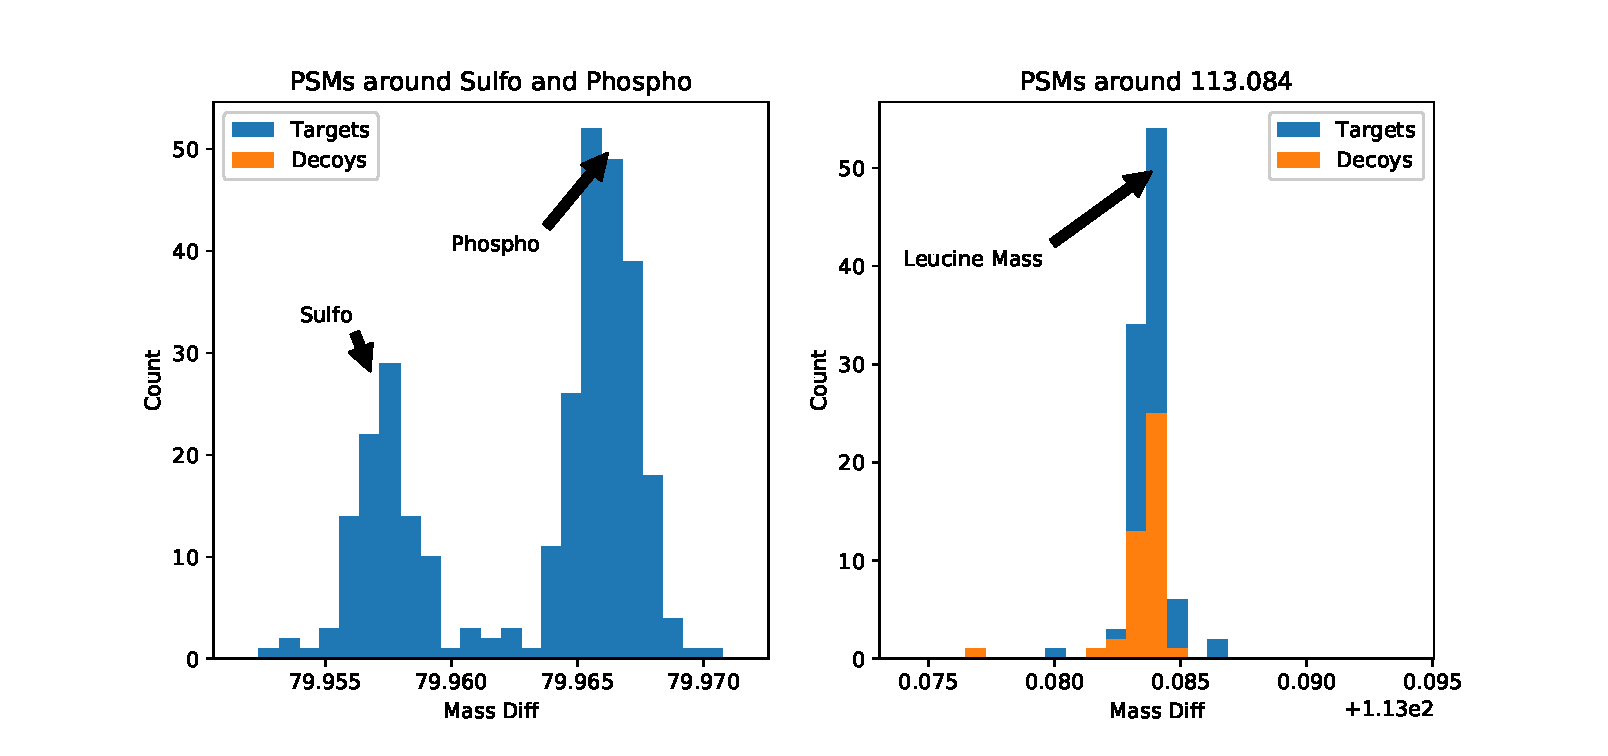
\includegraphics[scale=0.6]{figure_3peaks}
\end{figure}

We identified the property of some specific mass shifts that correspond to anomalously high false discovery rates: these mass shifts correspond precisely to various combinations of residue mass additions and removals.

Mass windows provide an mechanism to exclude these problematic mass shifts from a wide-mass search by employing a interval search.

\subsection{Discovery of Modifications not in Database}

Previously described wide mass search strategies for discovery and localization of unknown modifications benefit from using alternative, carefully designed search modes based on interval and notch searches.
We discovered that limiting mass shifts to a lower bound of -187 Da (corresponding to the largest mass difference that could be attributed to loss of a single residue, Tryptophan), and no upper bound, is an important step in eliminating spurious PSMs.
Furthermore, treating highly suspect mass shifts corresponding to residue additions/substitutions/deletions in a separate notch search with individualized false discovery rate estimates is beneficial.
An automated tool built into MetaMorpheus allows confidently identifying novel modifications based on these search results.

We describe the heuristic approach for augmenting the modification database and the final notch list.
After the conclusion of the search, the PSMs within 1\% FDR are selected, and the corresponding mass differences are grouped into peaks, which are categorized into one of the following categories:
\begin{itemize}
\item \textit{No mass error} Exact match (within a certain noise tolerance) between the peptide corresponding to the MS2 fragmentation and the reported precursor monoisotopic mass.
\item \textit{Monoisotopic error} Peaks around values such as 1.003, 2.006, 3.009 (average differences in mass between the monoisotopic peaks and the first few isotope peks). These correspond to having misidentified the monoisotopic peak in the preprocessing deconvolution step. In this case, the identified peptide is still correct. 
\item \textit{Exact PTM or Adduct Masses}e.g. 42.010 for Acetylation or 21.981 for Sodium adduct. In this analysis, there is no conceptual difference between PTMs and adducts: both are observed simply as mass differences between the identified peptide and the precursor mass.  These peaks are further classified into
\begin{itemize}
\item Localizeable - e.g. Methylation. There is evidence for the modification in the MS2 spectrum: the corresponding peaks are shifted by an appropriate amount. 
\item Labile - e.g. Sulfonation. There is no evidence of the modification in the fragmentation spectrum. 
\item Either Localizeable or Labile, e.g. Phosphorylation. Sometimes there is evidence of it in the fragmentation spectrum, and sometimes there is not. 
\end{itemize}
\item Amino acid removals, additions or substitutions.
\item Modification dependent mass shifts - these peaks occur only in presence of certain modifications in the identified peptide. 	E.g. -15.995 in presence of an identified oxidation, or -79.966 in presence on an identified phosphorylation. 
\item Combinations of any of the above, e.g. 1.987 for combination of a monoisotopic error and a deamidation. Some of these combinations occur frequently, and it is crucial to account for them. 
\end{itemize}

An automated script analyzes each identified peak, and provides clues to the nature of the peak. For every peak, a profile is automatically generated.
It includes the total number of unique peptides associated with the mass shift, the fraction of decoys, mass match with any known entry in the Unimod or UniProt database, mass match to an amino acid addition/removal combination, mass match to a combination of higher frequency peaks, fraction of localizable targets, localization residues and/or termini, and presence of any modifications in the matched peptides.
We follow the following procedure to classify mass shift peaks. 
1.	A z score is computed for the fraction of decoys in the peak, comparing with 1\%FDR. If it corresponds to p>0.05, we do not include this peak in the analysis, because there is no sufficient confidence it produces legitimate results.
2.	

An attempted localization of the mass difference is automatically performed on every peptide-spectrum match. We carefully examine the mass differences with a localization fraction greater than 0.2, and attempt to deduce the chemical formula, specificity sites and positions within a peptide.
Once a determination has been made, we add the new modification type to the modifications list.
An example output of this step is:
 

The improvements of using a Comb search instead of an Open search are two-fold. We summarize the differences in Table 2.
	Open Search	Comb Search
Search Time	54.36 hrs	29.66 hrs
 
The improvement in the discernibility of PTMs is apparent when running a comb search on calibrated vs uncalibrated spectra files. Specifically, the discernibility of PTMs with similar mass errors (ones that are only different because of the mass defect).
This was not really possible previously.
In the current run, Sulfation and Phosphorylation are readily distinguishable.
We present the numbers for the example below in the step 5 numerical validation section.
OPEN SEARCH CASE STUDY
Introduction of the comb search instead of an open search is motivated by a careful review of the Unimod database.
Known modifications with mass difference within 200 Daltons have values that are within [-0.1, 0.2] of every integer.
This interval choice stems from the mass defect in the primary isotope of the common elements.
PTM combinations also have this property.
We tested multiple search strategies in a search for one that gives the smallest number of false positives. 
\subsubsection{Known Modification Confirmation Case Study}

Confirmation of the properties of Sodium Adducts, Phosphorylation and Sulfonation.
\subsubsection{Glycans Case Study}
Proteins that contain modifications such as Hexose, HexNAC, and similar ones are interesting.
The uniprot database only lists some possible sites for such modifications, but does not specify the actual type, thus creating ambiguity regarding the type of the modification.
The new modification discovery workflow is well suited to identify such proteins.
Table~\ref{tbl:glyco} lists the automatically identified glyco modification masses and identities, sorted by frequency of occurence. 

\begin{table}[]
\centering
\caption{Glyco}
\label{tbl:glyco}
\begin{tabular}{lll}
MassShift & Count & UnimodID                        \\
\hline
203.079   & 30    & HexNAc                          \\
162.052   & 18    & Hex                             \\
876.322   & 10    & Hex(2)HexNAc(2)dHex(1)          \\
656.228   & 8     & Hex(1)HexNAc(1)NeuAc(1)         \\
365.132   & 8     & Hex(1)HexNAc(1)                 \\
1216.422  & 8     & Hex(5)HexNAc(2)                 \\
730.265   & 6     & Hex(2)HexNAc(2)                 \\
1378.475  & 4     & Hex(6)HexNAc(2)                 \\
947.323   & 4     & Hex(1)HexNAc(1)NeuAc(2)         \\
963.317   & 3     & Hex(1)HexNAc(1)NeuAc(1)NeuGc(1) \\
178.047   & 3     & Galactosyl                      \\
1038.375  & 3     & dHex(1)Hex(3)HexNAc(2)          \\
146.058   & 2     & dHex                            \\
340.1     & 2     & Glucosylgalactosyl              \\
406.158   & 2     & HexNAc(2)                       \\
697.256   & 2     & HexNAc(2)NeuAc(1)               \\
672.223   & 2     & Hex(1)HexNAc(1)NeuGc(1)         \\
860.326   & 2     & Hex(1)HexNAc(2)dHex(2)         
\end{tabular}
\end{table}

 
\subsubsection{Novel Modification Case Study}


\subsection{Calibration}

The spectral calibration procedure consists of two steps: Step 1: A standard tolerance (e.g. 10 ppm) database search is performed on the dataset.
This yields a set of peptide identifications subject to a desired false discovery rate (e.g 1\%; based upon the target:decoy strategy (ref)).
Step 2:  The identifications from step 1 are used to extract peak matches from the spectra, and a calibration procedure is performed.
The calibration algorithm is described in detail in Supplementary Material 1.
A simple test of the calibration quality is to withhold some known peak matches from the inputs of the calibration software, and to determine if they have been shifted closer to the theoretically correct value.
We withheld 30\% of identifications, and measured the standard deviation and the average errors of the peak differences for the monoisotopic MS1 peaks with known charge states.
The average mass error went down from -3.67ppm to -0.15ppm in the jurkat dataset and from -3.32ppm for the mouse dataset.
The standard deviations decreased from 3.64ppm to 2.82ppm, and from 3.07ppm to 2.54ppm for the jurkat and mouse datasets respectively.
Figure 2 shows the clear improvement in the error for the withheld identified peptides, as a result of applying spectral calibration.

A 10 ppm narrow tolerance search produces matches with mass differences in ppm given in~\ref{fgr:figure1}.
The average and standard deviations along with 1, 2, and 3 standard deviation widths are given in Table~\ref{tbl:calib}.

\begin{table}
  \caption{Calibration Results: ppm Mass Differences}
  \label{tbl:calib}
  \begin{tabular}{llll}
    \hline
    & prior& after smooth & after rf  \\
    \hline
    stdev&	1.553	&1.039&	0.898 \\
	avg&	-3.148&	0.204&0.215\\
	68.3\% within	& [-4.701,-1.595 ]&	[-0.834,1.243	]&	[-0.683,1.114]\\
	95.4\% within&[	-6.254,	-0.042]&[	-1.873,2.282]&[	-1.581,	2.012]\\
	99.7\% within&	[-7.807,	1.511]&[	-2.912,3.321]&[	-2.479,	2.910]\\
    \hline
  \end{tabular}
\end{table}


\begin{figure}
  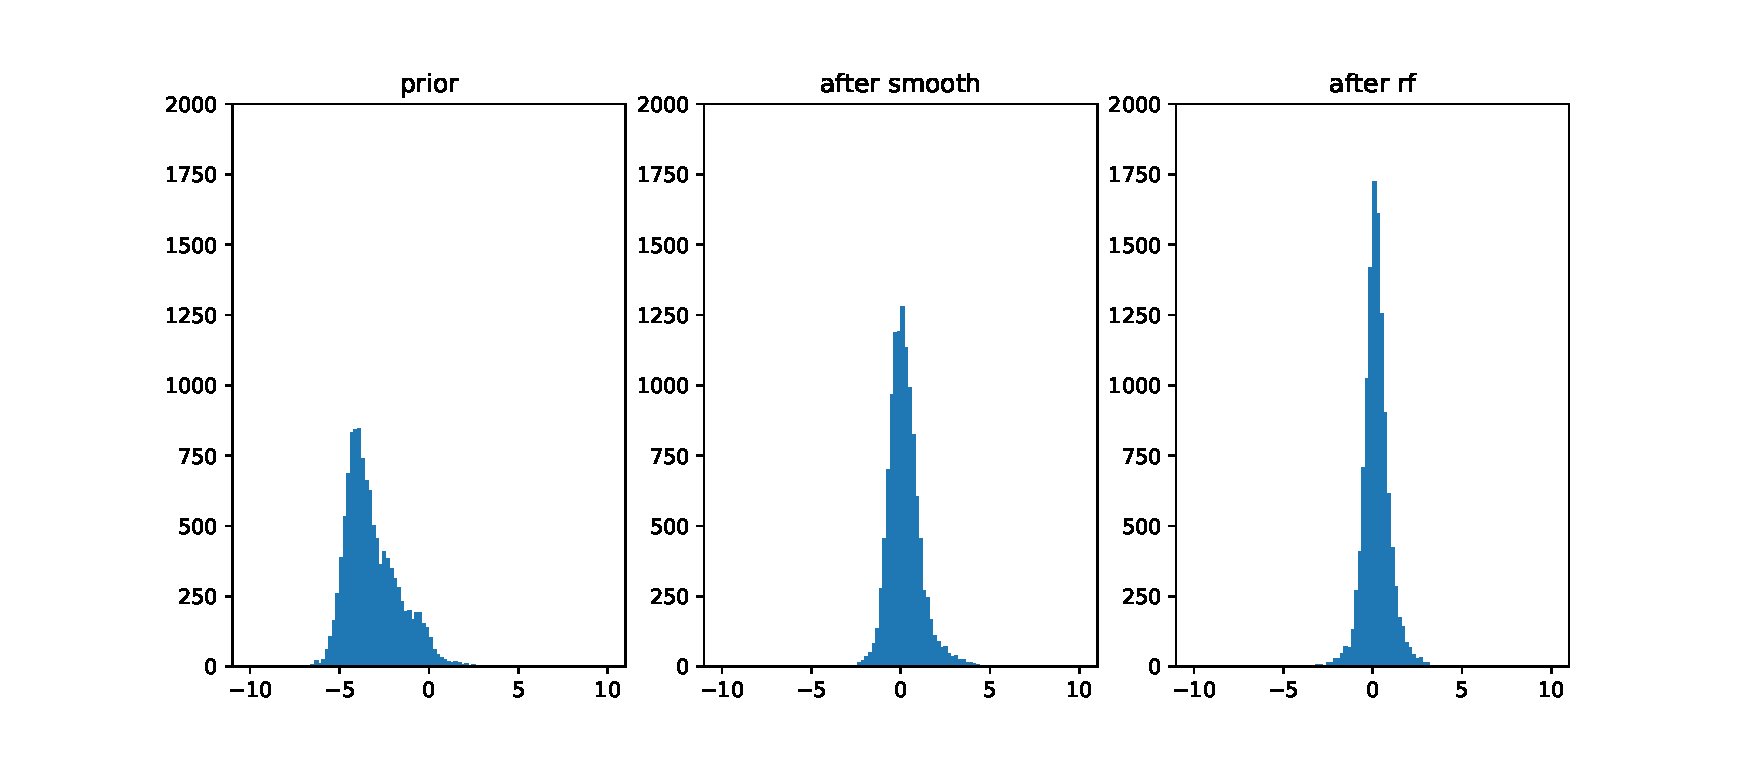
\includegraphics[scale=0.6]{figure_1.eps}
  \caption{An example figure}
  \label{fgr:figure1}
\end{figure}

%
%\subsection{References}
%
%The class makes various changes to the way that references are
%handled.  The class loads \textsf{natbib}, and also the
%appropriate bibliography style.  References can be made using
%the normal method; the citation should be placed before any
%punctuation, as the class will move it if using a superscript
%citation style
%\cite{Mena2000,Abernethy2003,Friedman-Hill2003,EuropeanCommission2008}.
%The use of \textsf{natbib} allows the use of the various citation
%commands of that package: \citeauthor{Abernethy2003} have shown
%something, in \citeyear{Cotton1999}, or as given by
%Ref.~\citenum{Mena2000}.  Long lists of authors will be
%automatically truncated in most article formats, but not in
%supplementary information or reviews \cite{Pople2003}. If you
%encounter problems with the citation macros, please check that
%your copy of \textsf{natbib} is up to date. The demonstration
%database file \texttt{achemso-demo.bib} shows how to complete
%entries correctly. Notice that ``\latin{et al.}'' is auto-formatted
%using the \texttt{\textbackslash latin} command.
%
%Multiple citations to be combined into a list can be given as
%a single citation.  This uses the \textsf{mciteplus} package
%\cite{Johnson1972,*Arduengo1992,*Eisenstein2005,*Arduengo1994}.
%Citations other than the first of the list should be indicated
%with a star. If the \textsf{mciteplus} package is not installed,
%the standard bibliography tools will still work but starred
%references will be ignored. Individual references can be referred
%to using \texttt{\textbackslash mciteSubRef}:
%``ref.~\mciteSubRef{Eisenstein2005}''.
%
%The class also handles notes to be added to the bibliography.  These
%should be given in place in the document \bibnote{This is a note.
%The text will be moved the the references section.  The title of the
%section will change to ``Notes and References''.}.  As with
%citations, the text should be placed before punctuation.  A note is
%also generated if a citation has an optional note.  This assumes that
%the whole work has already been cited: odd numbering will result if
%this is not the case \cite[p.~1]{Cotton1999}.

%\newpage
%
%\subsection{Floats}
%
%The example file also loads the optional \textsf{mhchem} package, so
%that formulas are easy to input: \texttt{\textbackslash ce\{H2SO4\}}
%gives \ce{H2SO4}.  See the use in the bibliography file (when using
%titles in the references section).
%
\begin{acknowledgement}

The authors thank \ldots
\end{acknowledgement}

\begin{suppinfo}

A listing of the contents of each file supplied as Supporting Information
should be included.
For instructions on what should be included in the
Supporting Information as well as how to prepare this material for
publications, refer to the journal's Instructions for Authors.

The following files are available free of charge.
\begin{itemize}
  \item Filename: brief description
  \item Filename: brief description
\end{itemize}

\end{suppinfo}

\newpage

\bibliography{citations}

\end{document}
